% Options for packages loaded elsewhere
\PassOptionsToPackage{unicode}{hyperref}
\PassOptionsToPackage{hyphens}{url}
%
\documentclass[
]{article}
\usepackage{amsmath,amssymb}
\usepackage{iftex}
\ifPDFTeX
  \usepackage[T1]{fontenc}
  \usepackage[utf8]{inputenc}
  \usepackage{textcomp} % provide euro and other symbols
\else % if luatex or xetex
  \usepackage{unicode-math} % this also loads fontspec
  \defaultfontfeatures{Scale=MatchLowercase}
  \defaultfontfeatures[\rmfamily]{Ligatures=TeX,Scale=1}
\fi
\usepackage{lmodern}
\ifPDFTeX\else
  % xetex/luatex font selection
\fi
% Use upquote if available, for straight quotes in verbatim environments
\IfFileExists{upquote.sty}{\usepackage{upquote}}{}
\IfFileExists{microtype.sty}{% use microtype if available
  \usepackage[]{microtype}
  \UseMicrotypeSet[protrusion]{basicmath} % disable protrusion for tt fonts
}{}
\makeatletter
\@ifundefined{KOMAClassName}{% if non-KOMA class
  \IfFileExists{parskip.sty}{%
    \usepackage{parskip}
  }{% else
    \setlength{\parindent}{0pt}
    \setlength{\parskip}{6pt plus 2pt minus 1pt}}
}{% if KOMA class
  \KOMAoptions{parskip=half}}
\makeatother
\usepackage{xcolor}
\usepackage[margin=1in]{geometry}
\usepackage{color}
\usepackage{fancyvrb}
\newcommand{\VerbBar}{|}
\newcommand{\VERB}{\Verb[commandchars=\\\{\}]}
\DefineVerbatimEnvironment{Highlighting}{Verbatim}{commandchars=\\\{\}}
% Add ',fontsize=\small' for more characters per line
\usepackage{framed}
\definecolor{shadecolor}{RGB}{248,248,248}
\newenvironment{Shaded}{\begin{snugshade}}{\end{snugshade}}
\newcommand{\AlertTok}[1]{\textcolor[rgb]{0.94,0.16,0.16}{#1}}
\newcommand{\AnnotationTok}[1]{\textcolor[rgb]{0.56,0.35,0.01}{\textbf{\textit{#1}}}}
\newcommand{\AttributeTok}[1]{\textcolor[rgb]{0.13,0.29,0.53}{#1}}
\newcommand{\BaseNTok}[1]{\textcolor[rgb]{0.00,0.00,0.81}{#1}}
\newcommand{\BuiltInTok}[1]{#1}
\newcommand{\CharTok}[1]{\textcolor[rgb]{0.31,0.60,0.02}{#1}}
\newcommand{\CommentTok}[1]{\textcolor[rgb]{0.56,0.35,0.01}{\textit{#1}}}
\newcommand{\CommentVarTok}[1]{\textcolor[rgb]{0.56,0.35,0.01}{\textbf{\textit{#1}}}}
\newcommand{\ConstantTok}[1]{\textcolor[rgb]{0.56,0.35,0.01}{#1}}
\newcommand{\ControlFlowTok}[1]{\textcolor[rgb]{0.13,0.29,0.53}{\textbf{#1}}}
\newcommand{\DataTypeTok}[1]{\textcolor[rgb]{0.13,0.29,0.53}{#1}}
\newcommand{\DecValTok}[1]{\textcolor[rgb]{0.00,0.00,0.81}{#1}}
\newcommand{\DocumentationTok}[1]{\textcolor[rgb]{0.56,0.35,0.01}{\textbf{\textit{#1}}}}
\newcommand{\ErrorTok}[1]{\textcolor[rgb]{0.64,0.00,0.00}{\textbf{#1}}}
\newcommand{\ExtensionTok}[1]{#1}
\newcommand{\FloatTok}[1]{\textcolor[rgb]{0.00,0.00,0.81}{#1}}
\newcommand{\FunctionTok}[1]{\textcolor[rgb]{0.13,0.29,0.53}{\textbf{#1}}}
\newcommand{\ImportTok}[1]{#1}
\newcommand{\InformationTok}[1]{\textcolor[rgb]{0.56,0.35,0.01}{\textbf{\textit{#1}}}}
\newcommand{\KeywordTok}[1]{\textcolor[rgb]{0.13,0.29,0.53}{\textbf{#1}}}
\newcommand{\NormalTok}[1]{#1}
\newcommand{\OperatorTok}[1]{\textcolor[rgb]{0.81,0.36,0.00}{\textbf{#1}}}
\newcommand{\OtherTok}[1]{\textcolor[rgb]{0.56,0.35,0.01}{#1}}
\newcommand{\PreprocessorTok}[1]{\textcolor[rgb]{0.56,0.35,0.01}{\textit{#1}}}
\newcommand{\RegionMarkerTok}[1]{#1}
\newcommand{\SpecialCharTok}[1]{\textcolor[rgb]{0.81,0.36,0.00}{\textbf{#1}}}
\newcommand{\SpecialStringTok}[1]{\textcolor[rgb]{0.31,0.60,0.02}{#1}}
\newcommand{\StringTok}[1]{\textcolor[rgb]{0.31,0.60,0.02}{#1}}
\newcommand{\VariableTok}[1]{\textcolor[rgb]{0.00,0.00,0.00}{#1}}
\newcommand{\VerbatimStringTok}[1]{\textcolor[rgb]{0.31,0.60,0.02}{#1}}
\newcommand{\WarningTok}[1]{\textcolor[rgb]{0.56,0.35,0.01}{\textbf{\textit{#1}}}}
\usepackage{graphicx}
\makeatletter
\def\maxwidth{\ifdim\Gin@nat@width>\linewidth\linewidth\else\Gin@nat@width\fi}
\def\maxheight{\ifdim\Gin@nat@height>\textheight\textheight\else\Gin@nat@height\fi}
\makeatother
% Scale images if necessary, so that they will not overflow the page
% margins by default, and it is still possible to overwrite the defaults
% using explicit options in \includegraphics[width, height, ...]{}
\setkeys{Gin}{width=\maxwidth,height=\maxheight,keepaspectratio}
% Set default figure placement to htbp
\makeatletter
\def\fps@figure{htbp}
\makeatother
\setlength{\emergencystretch}{3em} % prevent overfull lines
\providecommand{\tightlist}{%
  \setlength{\itemsep}{0pt}\setlength{\parskip}{0pt}}
\setcounter{secnumdepth}{-\maxdimen} % remove section numbering
\usepackage{setspace}\onehalfspacing
\ifLuaTeX
  \usepackage{selnolig}  % disable illegal ligatures
\fi
\IfFileExists{bookmark.sty}{\usepackage{bookmark}}{\usepackage{hyperref}}
\IfFileExists{xurl.sty}{\usepackage{xurl}}{} % add URL line breaks if available
\urlstyle{same}
\hypersetup{
  hidelinks,
  pdfcreator={LaTeX via pandoc}}

\author{}
\date{\vspace{-2.5em}}

\begin{document}

\hypertarget{eksamenssuxe6t-1}{%
\section{Eksamenssæt 1}\label{eksamenssuxe6t-1}}

\hypertarget{opgave-1---estimer-modellen-vha.-ols.-kommenter-puxe5-outputtet-og-fortolk-resultaterne}{%
\subsection{Opgave 1 - Estimer modellen vha. OLS. Kommenter på outputtet
og fortolk
resultaterne}\label{opgave-1---estimer-modellen-vha.-ols.-kommenter-puxe5-outputtet-og-fortolk-resultaterne}}

\begin{Shaded}
\begin{Highlighting}[]
\NormalTok{model1 }\OtherTok{=} \FunctionTok{lm}\NormalTok{(logsal }\SpecialCharTok{\textasciitilde{}}\NormalTok{ educ}\SpecialCharTok{+}\NormalTok{logbegin}\SpecialCharTok{+}\NormalTok{male}\SpecialCharTok{+}\NormalTok{minority)}
\FunctionTok{summary}\NormalTok{(model1)}
\end{Highlighting}
\end{Shaded}

\begin{verbatim}
## 
## Call:
## lm(formula = logsal ~ educ + logbegin + male + minority)
## 
## Residuals:
##       Min        1Q    Median        3Q       Max 
## -0.703137 -0.133323 -0.013904  0.117808  0.844933 
## 
## Coefficients:
##               Estimate Std. Error t value              Pr(>|t|)    
## (Intercept)  2.4134957  0.0439167 54.9562 < 0.00000000000000022 ***
## educ         0.0347858  0.0039348  8.8405 < 0.00000000000000022 ***
## logbegin     0.0300821  0.0015288 19.6767 < 0.00000000000000022 ***
## male         0.1280173  0.0200758  6.3767       0.0000000004339 ***
## minority    -0.0698858  0.0216829 -3.2231              0.001357 ** 
## ---
## Signif. codes:  0 '***' 0.001 '**' 0.01 '*' 0.05 '.' 0.1 ' ' 1
## 
## Residual standard error: 0.18983 on 469 degrees of freedom
## Multiple R-squared:  0.77368,    Adjusted R-squared:  0.77175 
## F-statistic: 400.83 on 4 and 469 DF,  p-value: < 0.000000000000000222
\end{verbatim}

Alle estimater er signifikante på 0,1\% bortset fra ``Minority'', som er
signifikant på 1\%.

F-testen afvises grundet den lave p-værdi angivet ved \textless{}
0.000000000000000222, hvilket vil sige at variablene er ``jointly
significant'', da nulhypotesen i F-testen, \(H_0 = \beta_{1,2,3,4} = 0\)
afvises. Under antagelse af, at alle andre variable er faste, vil en
stigning i ``educ'' (uddannelse) på 1, medfører en stigning i lønnen på
3,5\%. Et ekstra års uddannelse vil altså øge lønnen med 3,5\%. Samme
princip er gældende for de tre andre variable ``logbegin'', ``male'',
``minority''. Derudover angiver ovenstående model at \(R^2 = 0.77\),
hvilket vil sige at dataen passer relativt godt til den estimerede
model.

\hypertarget{opgave-2---udfuxf8r-grafisk-modelkontrol}{%
\subsection{Opgave 2 - Udfør grafisk
modelkontrol}\label{opgave-2---udfuxf8r-grafisk-modelkontrol}}

For at udføre grafisk kontrol opstilles en række plots som beskrives
nedenfor.

\begin{Shaded}
\begin{Highlighting}[]
\FunctionTok{par}\NormalTok{(}\AttributeTok{mfrow=}\FunctionTok{c}\NormalTok{(}\DecValTok{2}\NormalTok{,}\DecValTok{2}\NormalTok{))}
\FunctionTok{plot}\NormalTok{(model1)}
\end{Highlighting}
\end{Shaded}

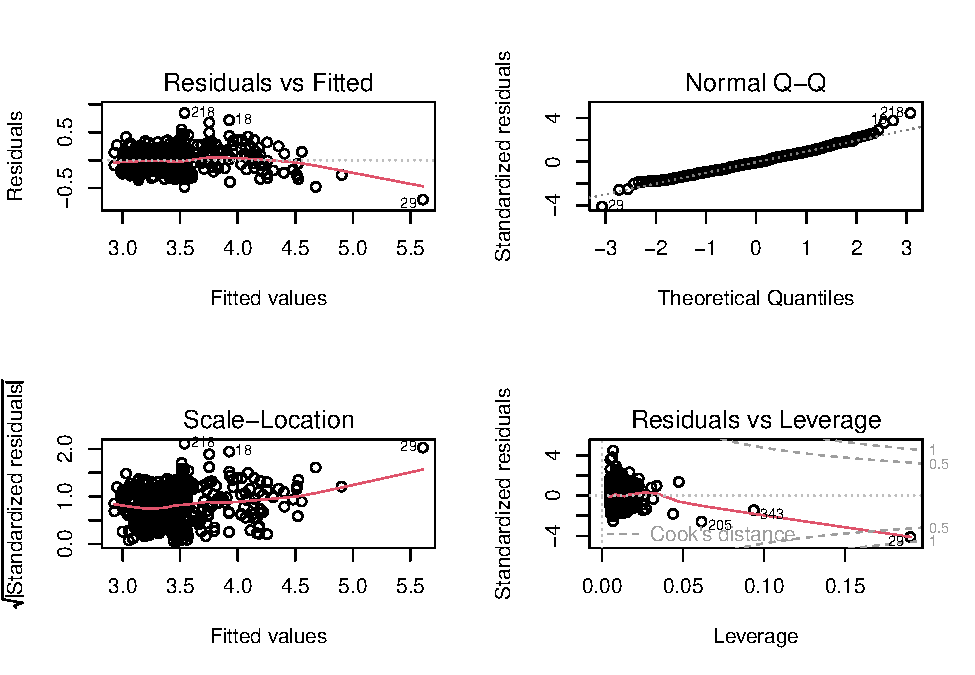
\includegraphics{Eksamensopgave-1_files/figure-latex/unnamed-chunk-3-1.pdf}
Ovenstående er udført grafisk modelkontrol. ``Residuals vs.~Fitted''
viser at residualerne ikke er spredte, hvilket er indikation på at der
ikke er tale om et ``non-linear relationsship''. Dog er den røde linje
her næsten vandret (med undtagelse af den sidste del fra 4,5 på aksen
for fitted values er linjens hældning negativ), hvilket kunne være tegn
homoskedasticitet og dermed være tegn på et ``linear relationship''.
``Q-Q plot'' viser at residualerne tilnærmelsesvist følger en ret linje,
og derfor antages formodes at være normalfordelt. ``Scale-Location''
belyser, at der er en skæv ``scale-location'', hvilket kan indikerer at
der er tale om heteroskedasticitet for modellen. Ideelt ønskes, at den
røde linje er vandret samt at residualpunkterne er spredt og tilfældigt
fordelt. ``Resudials vs.~Leverage'' tydeliggøre problematikken
vedrørende outliers. Y-aksen angiver de standardiseret residualer givet
ved \(\frac {e}{se}\), mens x-aksen angiver viser ``leverage'' som måler
hvor stor indflydelse en observation har på estimaternes for
regressionens koefficienter. De stiblede linjer viser de forskellige
niveauer for Cook's distance, som viser hvorvidt en outlier har stor
betydning for estimationen for regressionens koefficienter. Hvis Cook's
distancen for en observation er større end 1, anses den for at være
indflydelsesrig for estimationen. I modellen ses tre outliers, 205, 343
og 029. Her ligger de to førstnævnte indenfor Cook's distance på 0,5
vurderes til at have lav indflydelse, mens 029 ligger på en Cook's
distance imellem 0,5 og 1, hvilket heller ikke vurderes til at have den
store effekt på regressionens estimater.

Mangler noget med cook's distance - er det tilstrækkeligt? ``Dog er den
røde linje her næsten vandret, hvilket kunne være tegn på det
modsatte.''? - er det tilstrækkeligt?

\hypertarget{opgave-3---test-for-heteroskedasticitet-vha.-breusch-pagan-testen-og-specialudgaven-af-white-testen}{%
\subsection{Opgave 3 - Test for heteroskedasticitet vha.
Breusch-Pagan-testen og specialudgaven af
White-testen}\label{opgave-3---test-for-heteroskedasticitet-vha.-breusch-pagan-testen-og-specialudgaven-af-white-testen}}

For at teste for heteroskedasticitet udføres BP-testen samt
specialudgaven af White-testen. Her udføres både BP-testen både manuelt
og vha. funktionen i R. BP-testen udføres ved at kvadrere fejlledet i
den oprindelige regression, hvorefter denne opstilles som en funktion af
de uafhængige variable fra den oprindelige regression. Der udføres en
F-test eller LM-test for at estimere p-værdien, og hvis denne er under
det valgte siginifikansniveau afvises nullhypotesen. White-testen
udføres også ved at opstille en regression for det kvadreret fejlled.
Dog opstilles denne med de uafængige variable, de kvadrerede uafhængige
variable samt krydsprodukterne af de uafhængige variable. Igen udføres
en F-test eller LM-test for at vurdere hvorvidt nulhypotesen afvises
eller accepteres. SKAL KAN REDEGØRES FOR TESTEN?
\[H_0: homoskedasticitet\] Hvis p-værdien er lav i BP-testen/F-test vil
\(H_0\) afvises hvorfor der antages at være heteroskedasticitet.

\begin{Shaded}
\begin{Highlighting}[]
\NormalTok{u }\OtherTok{=} \FunctionTok{resid}\NormalTok{(model1)}
\NormalTok{u2 }\OtherTok{=}\NormalTok{ u}\SpecialCharTok{\^{}}\DecValTok{2}
\NormalTok{model1u }\OtherTok{=} \FunctionTok{lm}\NormalTok{(u2 }\SpecialCharTok{\textasciitilde{}}\NormalTok{ educ}\SpecialCharTok{+}\NormalTok{logbegin}\SpecialCharTok{+}\NormalTok{male}\SpecialCharTok{+}\NormalTok{minority) }\CommentTok{\#Test for heteroskedasticitet}
\FunctionTok{summary}\NormalTok{(model1u)}
\end{Highlighting}
\end{Shaded}

\begin{verbatim}
## 
## Call:
## lm(formula = u2 ~ educ + logbegin + male + minority)
## 
## Residuals:
##       Min        1Q    Median        3Q       Max 
## -0.093988 -0.026914 -0.015922  0.009181  0.679610 
## 
## Coefficients:
##                Estimate  Std. Error t value   Pr(>|t|)    
## (Intercept) -0.00226560  0.01435324 -0.1578     0.8746    
## educ         0.00030711  0.00128602  0.2388     0.8114    
## logbegin     0.00214957  0.00049966  4.3020 0.00002061 ***
## male        -0.00189537  0.00656134 -0.2889     0.7728    
## minority    -0.00806218  0.00708658 -1.1377     0.2558    
## ---
## Signif. codes:  0 '***' 0.001 '**' 0.01 '*' 0.05 '.' 0.1 ' ' 1
## 
## Residual standard error: 0.062041 on 469 degrees of freedom
## Multiple R-squared:  0.077789,   Adjusted R-squared:  0.069923 
## F-statistic: 9.8901 on 4 and 469 DF,  p-value: 0.00000010889
\end{verbatim}

Da nulhypotesen i F-testen afvises angiver det, at der er
heteroskedasticitet i modellen. Ved at bruge \(\chi^2\) i stedet for
F-test findes Breusch-Pagan testen.

\begin{Shaded}
\begin{Highlighting}[]
\NormalTok{lm\_chi }\OtherTok{=} \FloatTok{0.077789}\SpecialCharTok{*}\DecValTok{474} \CommentTok{\#BP{-}test}
\DecValTok{1}\SpecialCharTok{{-}}\FunctionTok{pchisq}\NormalTok{(lm\_chi, }\DecValTok{4}\NormalTok{) }\CommentTok{\#p{-}værdien for chi{-}square}
\end{Highlighting}
\end{Shaded}

\begin{verbatim}
## [1] 0.00000019140651
\end{verbatim}

\begin{Shaded}
\begin{Highlighting}[]
\FunctionTok{bptest}\NormalTok{(model1)}
\end{Highlighting}
\end{Shaded}

\begin{verbatim}
## 
##  studentized Breusch-Pagan test
## 
## data:  model1
## BP = 36.8719, df = 4, p-value = 0.00000019142
\end{verbatim}

BP-værdien på 36.8719 indikerer, at variansen af residualerne ikke er
konstant, hvilket også bekræftes ved den lave p-værdi for chi-square.
Med den lave p-værdi, kan \(H_0\) afvises, hvorfor det tyder på, at der
findes heteroskedasticitet.

White-test med fitted værdier\textbackslash{} Her benyttes residualer i
anden som regresseres på de fitted værdier af modellen og de fitted
værdier i anden for at belyse lineære og ikke-lineære forhold mellem de
uafhængige variable og residualerne.

\begin{Shaded}
\begin{Highlighting}[]
\NormalTok{white }\OtherTok{=} \FunctionTok{lm}\NormalTok{(u2 }\SpecialCharTok{\textasciitilde{}} \FunctionTok{predict}\NormalTok{(model1) }\SpecialCharTok{+} \FunctionTok{I}\NormalTok{(}\FunctionTok{predict}\NormalTok{(model1)}\SpecialCharTok{\^{}}\DecValTok{2}\NormalTok{))}
\FunctionTok{summary}\NormalTok{(white)}
\end{Highlighting}
\end{Shaded}

\begin{verbatim}
## 
## Call:
## lm(formula = u2 ~ predict(model1) + I(predict(model1)^2))
## 
## Residuals:
##       Min        1Q    Median        3Q       Max 
## -0.102842 -0.026861 -0.016738  0.007690  0.681670 
## 
## Coefficients:
##                       Estimate Std. Error t value  Pr(>|t|)    
## (Intercept)           0.510248   0.175199  2.9124 0.0037571 ** 
## predict(model1)      -0.300244   0.094263 -3.1852 0.0015426 ** 
## I(predict(model1)^2)  0.046678   0.012562  3.7157 0.0002269 ***
## ---
## Signif. codes:  0 '***' 0.001 '**' 0.01 '*' 0.05 '.' 0.1 ' ' 1
## 
## Residual standard error: 0.061276 on 471 degrees of freedom
## Multiple R-squared:  0.096563,   Adjusted R-squared:  0.092727 
## F-statistic: 25.171 on 2 and 471 DF,  p-value: 0.000000000041107
\end{verbatim}

Igen afvises nulhypotesen i F-testen og der antages derfor at være
heteroskedasticitet. Både \(\hat{y}\) og \(\hat{y}^2\) er signifikante i
testen, så det kan ikke siges hvorvidt der er et lineært eller
ikke-lineært forhold.

\hypertarget{opgave-4---beregn-robuste-standardfejl-for-modellen-og-sammenlign-med-resultaterne-i-spuxf8rgsmuxe5l-1}{%
\subsection{Opgave 4 - Beregn robuste standardfejl for modellen og
sammenlign med resultaterne i spørgsmål
1}\label{opgave-4---beregn-robuste-standardfejl-for-modellen-og-sammenlign-med-resultaterne-i-spuxf8rgsmuxe5l-1}}

\begin{Shaded}
\begin{Highlighting}[]
\NormalTok{model1robust }\OtherTok{\textless{}{-}} \FunctionTok{coeftest}\NormalTok{(model1, }\AttributeTok{vcov =} \FunctionTok{vcovHC}\NormalTok{(model1, }\AttributeTok{type =} \StringTok{"HC0"}\NormalTok{))}
\FunctionTok{screenreg}\NormalTok{(}\FunctionTok{list}\NormalTok{(}\AttributeTok{OLS =}\NormalTok{ model1, }\AttributeTok{OLS\_robust\_se =}\NormalTok{ model1robust), }\AttributeTok{digits =} \DecValTok{4}\NormalTok{)}
\end{Highlighting}
\end{Shaded}

\begin{verbatim}
## 
## ========================================
##              OLS           OLS_robust_se
## ----------------------------------------
## (Intercept)    2.4135 ***   2.4135 ***  
##               (0.0439)     (0.0399)     
## educ           0.0348 ***   0.0348 ***  
##               (0.0039)     (0.0046)     
## logbegin       0.0301 ***   0.0301 ***  
##               (0.0015)     (0.0030)     
## male           0.1280 ***   0.1280 ***  
##               (0.0201)     (0.0214)     
## minority      -0.0699 **   -0.0699 ***  
##               (0.0217)     (0.0189)     
## ----------------------------------------
## R^2            0.7737                   
## Adj. R^2       0.7718                   
## Num. obs.    474                        
## ========================================
## *** p < 0.001; ** p < 0.01; * p < 0.05
\end{verbatim}

Den venstre kolonne udgør resultaterne fra opgave 1, mens den højre
kolonne viser samme estimater men med robuste standardafvigelser. Der
findes en lille ændring i signifikansniveauet, hvor ``minority'' er
signifikant på et højere niveau, hvilket skyldes den lavere
standardafvigelse.

\hypertarget{opgave-5---test-hypotesen-h0-beta_2-1-mod-alternativet-h1-beta_2-neq-1}{%
\subsection{\texorpdfstring{Opgave 5 - Test hypotesen H0:
\(\beta_2 = 1\) mod alternativet H1:
\(\beta_2 \neq 1\)}{Opgave 5 - Test hypotesen H0: \textbackslash beta\_2 = 1 mod alternativet H1: \textbackslash beta\_2 \textbackslash neq 1}}\label{opgave-5---test-hypotesen-h0-beta_2-1-mod-alternativet-h1-beta_2-neq-1}}

T-scoren beregnes med følgende formel
\[T = \frac{\hat{\beta}_j-\beta_j}{se(\hat{\beta}_j)}\] Der vil blive
brugt robust se \textbackslash{} \(a_j\) er H0

\begin{Shaded}
\begin{Highlighting}[]
\CommentTok{\#summary(model1)}
\NormalTok{t }\OtherTok{=}\NormalTok{ (}\FloatTok{0.03008211}\DecValTok{{-}1}\NormalTok{) }\SpecialCharTok{/} \FloatTok{0.00296699}
\NormalTok{t}
\end{Highlighting}
\end{Shaded}

\begin{verbatim}
## [1] -326.90299
\end{verbatim}

\begin{Shaded}
\begin{Highlighting}[]
\CommentTok{\#kritiske værdier}
\NormalTok{alpha }\OtherTok{=} \FunctionTok{c}\NormalTok{(}\FloatTok{0.05}\NormalTok{, }\FloatTok{0.01}\NormalTok{)}
\FunctionTok{qt}\NormalTok{(}\DecValTok{1}\SpecialCharTok{{-}}\NormalTok{alpha}\SpecialCharTok{/}\DecValTok{2}\NormalTok{, }\DecValTok{469}\NormalTok{)}
\end{Highlighting}
\end{Shaded}

\begin{verbatim}
## [1] 1.9650350 2.5863526
\end{verbatim}

\begin{Shaded}
\begin{Highlighting}[]
\CommentTok{\#P{-}værdier}
\FunctionTok{pt}\NormalTok{(}\SpecialCharTok{{-}}\FunctionTok{abs}\NormalTok{(t), }\DecValTok{469}\NormalTok{)}
\end{Highlighting}
\end{Shaded}

\begin{verbatim}
## [1] 0
\end{verbatim}

De kritiske værdier for 5\% og og 1\% er henholdsvis 1,96 og 2,59
hvorfor \(H_0\) afvises og \(\beta_2 \neq 1\). P-værdien rapporteres i R
som 0, da t-scoren er så lav at p-værdien er for lav til at vise.

\hypertarget{opgave-6---test-hypotesen-h0-beta_3-beta_4-0}{%
\subsection{\texorpdfstring{Opgave 6 - Test hypotesen H0:
\(\beta_3 = \beta_4 = 0\)}{Opgave 6 - Test hypotesen H0: \textbackslash beta\_3 = \textbackslash beta\_4 = 0}}\label{opgave-6---test-hypotesen-h0-beta_3-beta_4-0}}

F-test

\begin{Shaded}
\begin{Highlighting}[]
\FunctionTok{linearHypothesis}\NormalTok{(model1, }\FunctionTok{c}\NormalTok{(}\StringTok{"male=0"}\NormalTok{, }\StringTok{"minority=0"}\NormalTok{))}
\end{Highlighting}
\end{Shaded}

\begin{verbatim}
## Linear hypothesis test
## 
## Hypothesis:
## male = 0
## minority = 0
## 
## Model 1: restricted model
## Model 2: logsal ~ educ + logbegin + male + minority
## 
##   Res.Df     RSS Df Sum of Sq       F          Pr(>F)    
## 1    471 18.5322                                         
## 2    469 16.9002  2   1.63197 22.6445 0.0000000004092 ***
## ---
## Signif. codes:  0 '***' 0.001 '**' 0.01 '*' 0.05 '.' 0.1 ' ' 1
\end{verbatim}

\begin{Shaded}
\begin{Highlighting}[]
\CommentTok{\#model1a = lm(logsal \textasciitilde{} educ+logbegin)}
\CommentTok{\#waldtest(model1, model1a)}
\end{Highlighting}
\end{Shaded}

RSS (kan også kaldes SSR) beskriver residual sum of squares, som er
summen af de estimeret fejlled sat i anden, og hvis SSR = 0 er modellen
perfekt (\(R^2=1\)). Den meget lave p-værdi, som tilnærmelsesvist er
nul, gør at H0 kan afvises. Dette betyder, at estimaterne ``male'' eller
``minority'' er ``jointly significant'' og dermed i fællesskab
forskellig fra 0.

For at beregne F-statistic, kan der gøres brug af følgende formel:
\[F = \frac {(SSR_r - SSR_{ur}) /q}{SSR_{ur} / (n - k - 1)}\] Her
angiver \(r\) den begrænsede model, hvor \(\beta_3 = \beta_4 = 0\), mens
\(ur\) angiver den ubegrænsede model hvor alle variable indgår. \(q\) er
forskellen i frihedsgrader mellem de to modeller. \((n-k-1)\) er antal
frihedsgrader i den ubegrænset model, hvor \(n\) er antal observationer
og \(k\) er antal variable i modellen.\textbackslash{} Jf. ovenstående
er F-værdien 22.6445, hvilket vil sige at der ikke er stor sandsynlighed
for at de to estimater \(\beta_3\) og \(\beta_4\) er lig med nul. Derfor
vil mindst et af de to estimater have relevans for modellen.

\hypertarget{opgave-7---estimer-modellen-vha.-fgls-og-kommenter-puxe5-resultaterne}{%
\subsection{Opgave 7 - Estimer modellen vha. FGLS og kommenter på
resultaterne}\label{opgave-7---estimer-modellen-vha.-fgls-og-kommenter-puxe5-resultaterne}}

\begin{Shaded}
\begin{Highlighting}[]
\NormalTok{logu2 }\OtherTok{\textless{}{-}} \FunctionTok{log}\NormalTok{(}\FunctionTok{resid}\NormalTok{(model1)}\SpecialCharTok{\^{}}\DecValTok{2}\NormalTok{) }\CommentTok{\#I do everything in one command, i.e., obtain resid, square them, and log them}
\NormalTok{varreg}\OtherTok{\textless{}{-}}\FunctionTok{lm}\NormalTok{(logu2 }\SpecialCharTok{\textasciitilde{}}\NormalTok{ educ}\SpecialCharTok{+}\NormalTok{logbegin}\SpecialCharTok{+}\NormalTok{male}\SpecialCharTok{+}\NormalTok{minority)}
\NormalTok{w }\OtherTok{\textless{}{-}} \FunctionTok{exp}\NormalTok{(}\FunctionTok{fitted}\NormalTok{(varreg))}
\NormalTok{model2fgls }\OtherTok{=} \FunctionTok{lm}\NormalTok{(logsal }\SpecialCharTok{\textasciitilde{}}\NormalTok{ educ}\SpecialCharTok{+}\NormalTok{logbegin}\SpecialCharTok{+}\NormalTok{male}\SpecialCharTok{+}\NormalTok{minority, }\AttributeTok{weight=}\DecValTok{1}\SpecialCharTok{/}\NormalTok{w)}
\FunctionTok{summary}\NormalTok{(model2fgls)}
\end{Highlighting}
\end{Shaded}

\begin{verbatim}
## 
## Call:
## lm(formula = logsal ~ educ + logbegin + male + minority, weights = 1/w)
## 
## Weighted Residuals:
##      Min       1Q   Median       3Q      Max 
## -4.62175 -1.38632 -0.14585  1.16367  9.10789 
## 
## Coefficients:
##               Estimate Std. Error t value              Pr(>|t|)    
## (Intercept)  2.4102704  0.0424302 56.8056 < 0.00000000000000022 ***
## educ         0.0254139  0.0038199  6.6530      0.00000000008025 ***
## logbegin     0.0387641  0.0020525 18.8865 < 0.00000000000000022 ***
## male         0.1021576  0.0188085  5.4315      0.00000008991339 ***
## minority    -0.0633470  0.0182882 -3.4638             0.0005814 ***
## ---
## Signif. codes:  0 '***' 0.001 '**' 0.01 '*' 0.05 '.' 0.1 ' ' 1
## 
## Residual standard error: 1.9092 on 469 degrees of freedom
## Multiple R-squared:  0.73271,    Adjusted R-squared:  0.73043 
## F-statistic: 321.42 on 4 and 469 DF,  p-value: < 0.000000000000000222
\end{verbatim}

\begin{Shaded}
\begin{Highlighting}[]
\FunctionTok{bptest}\NormalTok{(model2fgls)}
\end{Highlighting}
\end{Shaded}

\begin{verbatim}
## 
##  studentized Breusch-Pagan test
## 
## data:  model2fgls
## BP = 56179.2, df = 4, p-value < 0.000000000000000222
\end{verbatim}

\begin{Shaded}
\begin{Highlighting}[]
\FunctionTok{bptest}\NormalTok{(model1)}
\end{Highlighting}
\end{Shaded}

\begin{verbatim}
## 
##  studentized Breusch-Pagan test
## 
## data:  model1
## BP = 36.8719, df = 4, p-value = 0.00000019142
\end{verbatim}

Det ses hvordan alle koefficienter er statistisk signifikante på 0,1\%.
Desuden har modellen en høj forklaringsgrad på \(R^2 = 0,73\). De
relativt lave standard fejl i modellen indikerer præcise estimater.
T-værdierne udgør alle høje værdier, og disse kan sammen med de lave
p-værdier indikere, at den enkelte variable har en stærk effekt på den
afhængige variable.

\hypertarget{opgave-8---har-fgls-estimationen-taget-huxf8jde-for-al-heteroskedasticiteten}{%
\subsection{Opgave 8 - Har FGLS estimationen taget højde for al
heteroskedasticiteten?}\label{opgave-8---har-fgls-estimationen-taget-huxf8jde-for-al-heteroskedasticiteten}}

I ovenstående opgave 3 blev det tydeligt, at det signifikante resultat
fra Breusch-Pagan testen indikerede, at modellen indeholdte
heteroskedasticitet, hvilket er en god årsag til at benytte sig at FGLS
estimationen. Denne tager nemlig højde for heteroskedasticitet i
modellen, ved at omforme fejlledende så de bliver homoskedastiske
(konstant varians). Anvendelsen af FGLS gør modellen mere præcis, end de
resultater som opnås ved almindelig OLS, specielt når der er stærk
heteroskedasticitet til stede. Det kan dog ikke udelukkes, at der efter
FGLS estimationen ikke er mere heteroskedasticitet, og derfor kan der
udeføres en BP-test eller White-test.

\begin{Shaded}
\begin{Highlighting}[]
\NormalTok{u2 }\OtherTok{=} \FunctionTok{resid}\NormalTok{(model2fgls)}\SpecialCharTok{\^{}}\DecValTok{2}
\NormalTok{model2fgls\_u }\OtherTok{=} \FunctionTok{lm}\NormalTok{(u2 }\SpecialCharTok{\textasciitilde{}}\NormalTok{ educ}\SpecialCharTok{+}\NormalTok{logbegin}\SpecialCharTok{+}\NormalTok{male}\SpecialCharTok{+}\NormalTok{minority, }\AttributeTok{weight=}\DecValTok{1}\SpecialCharTok{/}\NormalTok{w)}
\FunctionTok{summary}\NormalTok{(model2fgls\_u)}
\end{Highlighting}
\end{Shaded}

\begin{verbatim}
## 
## Call:
## lm(formula = u2 ~ educ + logbegin + male + minority, weights = 1/w)
## 
## Weighted Residuals:
##      Min       1Q   Median       3Q      Max 
## -0.67542 -0.27943 -0.15665  0.08774  7.63779 
## 
## Coefficients:
##                Estimate  Std. Error t value  Pr(>|t|)    
## (Intercept) -0.00947968  0.01391304 -0.6814 0.4959851    
## educ         0.00033225  0.00125257  0.2653 0.7909283    
## logbegin     0.00260649  0.00067301  3.8729 0.0001228 ***
## male        -0.00208665  0.00616739 -0.3383 0.7352606    
## minority    -0.01028243  0.00599677 -1.7147 0.0870679 .  
## ---
## Signif. codes:  0 '***' 0.001 '**' 0.01 '*' 0.05 '.' 0.1 ' ' 1
## 
## Residual standard error: 0.62604 on 469 degrees of freedom
## Multiple R-squared:  0.070322,   Adjusted R-squared:  0.062393 
## F-statistic: 8.8689 on 4 and 469 DF,  p-value: 0.00000065587
\end{verbatim}

Da nulhypotesen i F-testen afvises angiver det, at der stadig er
heteroskedasticitet i modellen trods brug af FGLS. Ved at bruge
\(\chi^2\) i stedet for F-test findes Breusch-Pagan testen.

\begin{Shaded}
\begin{Highlighting}[]
\NormalTok{lm\_chi }\OtherTok{=} \FloatTok{0.070322}\SpecialCharTok{*}\DecValTok{474} \CommentTok{\#BP{-}test}
\DecValTok{1}\SpecialCharTok{{-}}\FunctionTok{pchisq}\NormalTok{(lm\_chi, }\DecValTok{4}\NormalTok{) }\CommentTok{\#p{-}værdien for chi{-}square}
\end{Highlighting}
\end{Shaded}

\begin{verbatim}
## [1] 0.0000010210752
\end{verbatim}

Det signifikante resultat fra Breusch-Pagan testen indikerer, at
modellen stadig indeholder heteroskedasticitet.

\begin{Shaded}
\begin{Highlighting}[]
\NormalTok{white\_fgls }\OtherTok{=} \FunctionTok{lm}\NormalTok{(u2 }\SpecialCharTok{\textasciitilde{}} \FunctionTok{predict}\NormalTok{(model2fgls) }\SpecialCharTok{+} \FunctionTok{I}\NormalTok{(}\FunctionTok{predict}\NormalTok{(model2fgls)}\SpecialCharTok{\^{}}\DecValTok{2}\NormalTok{))}
\FunctionTok{summary}\NormalTok{(white\_fgls)}
\end{Highlighting}
\end{Shaded}

\begin{verbatim}
## 
## Call:
## lm(formula = u2 ~ predict(model2fgls) + I(predict(model2fgls)^2))
## 
## Residuals:
##       Min        1Q    Median        3Q       Max 
## -0.249472 -0.024409 -0.012184  0.010928  0.756636 
## 
## Coefficients:
##                           Estimate Std. Error t value              Pr(>|t|)    
## (Intercept)               1.977306   0.151048  13.091 < 0.00000000000000022 ***
## predict(model2fgls)      -1.116090   0.079147 -14.101 < 0.00000000000000022 ***
## I(predict(model2fgls)^2)  0.158614   0.010227  15.509 < 0.00000000000000022 ***
## ---
## Signif. codes:  0 '***' 0.001 '**' 0.01 '*' 0.05 '.' 0.1 ' ' 1
## 
## Residual standard error: 0.068177 on 471 degrees of freedom
## Multiple R-squared:  0.46438,    Adjusted R-squared:  0.46211 
## F-statistic: 204.18 on 2 and 471 DF,  p-value: < 0.000000000000000222
\end{verbatim}

White-testen viser ligeledes tegn på heteroskedasticitet, da p-værdien i
F-testen er tilnærmelsesvis nul.

\end{document}
